\documentclass[10pt,a4paper]{ltjsarticle}

\usepackage{graphicx}
\usepackage{amsmath,amssymb}
\usepackage{booktabs,subfig}
\usepackage{pifont}
\usepackage{url}
\usepackage{cite}
\usepackage{ulem}
\usepackage{siunitx}
\usepackage{float}
\usepackage{tcolorbox}
\usepackage{cancel}
\usepackage{color}
\renewcommand{\CancelColor}{\color{red}}

\usepackage{tikz}
\usepackage{circuitikz}
\usetikzlibrary{shadows}
\usetikzlibrary{calc}

\usepackage{luatexja-fontspec}
%\setmainfont[Ligatures=TeX]{TeXGyreTermes}
%\setsansfont[Ligatures=TeX]{TeXGyreHeros}
\setmainfont{TimesNewRoman}
\setsansfont{Arial}
\defaultjfontfeatures{Scale=1.0}
\setmainjfont[BoldFont=IPAexGothic]{IPAexMincho}
%\setmainjfont[BoldFont=HiraMinProN-W6]{HiraMinProN-W3}
%\setmainjfont[BoldFont=IPAexGothic]{KozMinPr6N-Light}
%\setmainjfont[BoldFont=IPAexGothic]{MS-PMincho}
\setsansjfont{IPAexGothic}
%\setsansjfont{MS-PGothic}
%\setsansjfont[BoldFont=HiraginoSans-W8]{HiraginoSans-W4}

\begin{document}
\title{シンクロトロン振動のほへと}
\author{吉本伸一}
\maketitle
\tableofcontents
\clearpage

\section{Synchrotron motion}
シンクロトロン蓄積リングでは、偏向電磁石によって分散 (dispersion) が発生する為、粒子の横方向と縦方向の運動が結合する。この結合が、リングを周回する粒子の縦方向の振動 (シンクロトロン振動) において重要な役割を演じる。
%シンクロトロン振動は基準粒子(設計軌道を設計速度で運動する粒子)に対する、到着時間と運動量偏差の振動である。

\subsection{Synchronous particle}
運動量$p_0$を持つ粒子が、基準軌道\footnote{粒子の運動量に対応して、一定の閉じた軌道 (閉軌道) が存在する。}\ を周期$T_0$で周回し、高周波加速空洞を同じ位相$\phi_s$で通過する時、このような粒子のことを同期粒子 (synchronous particle) と呼ぶ。同期粒子であるためには、周回周波数$f_0 (= 1/T_0)$と空洞のRF周波数$f_{RF}$の間に
%
\begin{equation}
    f_{RF} = h f_0
    \label{harmonic}
\end{equation}
%
という関係が必要である。整数$h$をharmonic numberと言い、周波数$f_{RF}$で加速できる最大の粒子数になる。この時、空洞の加速電圧は
%
\begin{equation}
    V_c (\phi) = V_0 \sin (\phi),\:\phi = \omega_{RF} t + \phi_s
\end{equation}
%
となる。図\ref{synchronous}は、$h=2$の時の空洞電圧と同期粒子の関係を表してる。

\begin{figure}[hbt]
    \begin{center}
      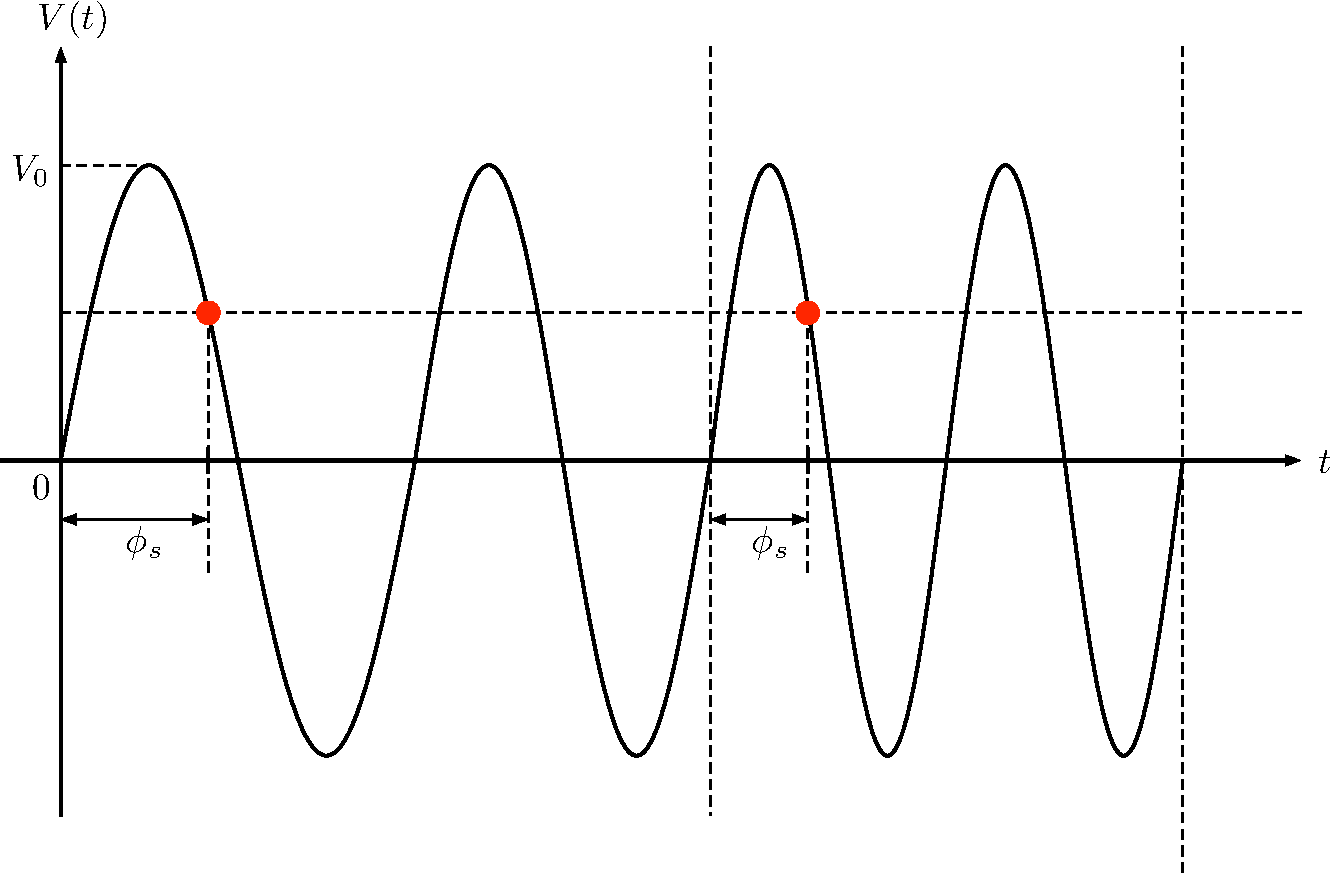
\includegraphics[width=15cm,clip]{synchronous.pdf}
      \caption{$f_{RF} = h f_0$ ($h=2$)}
      \label{synchronous}
    \end{center}
\end{figure}

\begin{tcolorbox}[title=\textgt{SuperKEKBにおける$f_{RF}$, $f_{0}$, $h$}の関係]
    SuperKEKBのリングでは、電子と陽電子は、ほぼ光速$c$で回っており、周長$C_0$は$\SI{3016.315}{\meter}$なので周回周波数$f_0$は
    %
    \begin{equation}
      f_0 = \frac{1}{T_0}=\frac{c}{C_0}=\frac{\SI{2.99792458e8}{\meter / \second}}{\SI{3016.315}{\meter}}=\SI{99.39}{\kilo\hertz} \notag
    \end{equation}
    %
    一方、RF周波数$f_{RF}$は$\SI{508.887}{\mega\hertz}$なので
    %
    \begin{equation}
        f_{RF} = 5120 f_0 \notag
    \end{equation}
    となり、確かに(\ref{harmonic})を満たしている。
\end{tcolorbox}

\subsection{各パラメータの運動量依存性}
同期粒子が平衡軌道$C_0$を速度$v_0$で周回する時、回転周期は
%
\begin{equation}
    T_0 = \frac{C_0}{v_0} \notag
\end{equation}
%
となる。今、$v = v_0 + \Delta v$, $C = C_0 + \Delta C$, $T=T_0 + \Delta T$
%
\begin{equation}
    T = T_0 + \Delta T = \frac{C_0 + \Delta C}{v_0 + \Delta v}\notag
\end{equation}
%
これより
%
\begin{align}
    & (T_0 + \Delta T)(v_0 + \Delta v) = C_0 + \Delta C \notag \\
    \Longleftrightarrow\quad & \underset{C_0}{\uwave{\cancel{v_0 T_0}}} + \Delta v T_0 + v_0 \Delta T +
    \underset{0}{\uwave{\cancel{\Delta v \Delta T}}}
    = \cancel{C_0} + \Delta C \notag \\
    \Longleftrightarrow\quad & v_0 \Delta T = \Delta C- \Delta v T_0 \notag \\
    \Longleftrightarrow\quad & \frac{\Delta T}{T_0} = \frac{\Delta C_0}{\underset{C_0}{\uwave{v_0 T_0}}} - \frac{\Delta v}{v_0} \notag
\end{align}
%
したがって、
%
\begin{equation}
    \frac{\Delta T}{T_0} = \frac{\Delta C}{C_0} - \frac{\Delta v}{v_0}
\end{equation}
%
この式より、回転周期の変動 ($\Delta T/T_0$) をもたらす要因として、軌道の長さの変動 ($\Delta C/C_0$) と粒子の速度の変動 ($\Delta v/v_0$)である事が分かる。


\subsection{Transition}
運動量偏差 (momentum deviation)
\begin{equation}
    \delta_p = \frac{p-p_0}{p_0}=\frac{\Delta p}{p_0}
\end{equation}
%
momentum compaction factor
%
\begin{equation}
    \frac{\Delta C}{C_0}=\alpha_p\frac{\Delta p}{p_0}=\alpha_p\delta_p
\end{equation}
%
phase slip factor
\begin{equation}
    \frac{\Delta T}{T_0}=\eta_p\frac{\Delta p}{p_0}
\end{equation}
%
\begin{equation}
    \frac{\Delta v}{v_0}=\frac{1}{\gamma_0^2}\frac{\Delta p}{p_0}
    \label{delta_v}
\end{equation}
%
したがって、
%
\begin{equation}
    \frac{\Delta T}{T_0} = \left(\alpha_p - \frac{1}{\gamma_0^2}\right)\frac{\Delta p}{p_0}
\end{equation}
%
\begin{tcolorbox}[title=相対論のおさらい]
    \begin{equation}
        E_0 = m_0 c^2 ,\quad E = \sqrt{E_0^2 + p^2 c^2} \tag{A.1}
    \end{equation}

    \begin{equation}
        \beta = \frac{v}{c}\,,\quad \gamma = \frac{E}{E_0}=\frac{m}{m_0}=\frac{1}{\sqrt{1-\beta^2}} \tag{A.2}
    \end{equation}

    \begin{equation}
        p = mv = \gamma m_0 v = \gamma m_0 \beta c \tag{A.3}
    \end{equation}

    \begin{equation}
        \frac{p}{E} = \frac{\gamma m_0 \beta c}{\gamma m_0 c^2} = \frac{\beta}{c} \tag{A.4}
    \end{equation}
\end{tcolorbox}
    %
\begin{tcolorbox}[title=式 (\ref{delta_v}) の導出]
    \begin{equation}
        \frac{dp}{dv} = m_0\frac{d}{dv}(\gamma v)
        = m_0 \left(\gamma + v \frac{d\gamma}{dv}\right) \notag
    \end{equation}
    %
    \begin{align}
        \frac{d\gamma}{dv} & = \frac{1}{c}\frac{d\gamma}{d\beta}= \frac{1}{c}\frac{d}{d\beta}\left(\frac{1}{\sqrt{1-\beta^2}}\right) \notag \\
        & = \frac{1}{c} \beta \underset{\gamma^{-2}}{\underbrace{(1-\beta^2)}}^{-\frac{3}{2}} = \frac{\beta \gamma^3}{c} \notag \\
        & = \frac{1}{c} \beta \underset{\gamma^{-2}}{\uwave{(1-\beta^2)}}^{-\frac{3}{2}} = \frac{\beta \gamma^3}{c} \notag
    \end{align}
    %
    これより、
    \begin{align}
        \frac{dp}{dv} & = m_0 \left(\gamma + v \frac{\beta \gamma^3}{c}\right)
        = m_0 \gamma \underset{\gamma^2}{\uwave{(1 + \beta^2 \gamma^2)}}
        = \frac{\gamma^2 p}{v} \notag
    \end{align}
    %
    \begin{equation}
        \therefore \quad \frac{dv}{v} = \frac{1}{\gamma^2}\frac{dp}{p} \tag{B.1}
    \end{equation}
\end{tcolorbox}
%
正の運動量圧縮率$\alpha_p>0$を持つ電磁石の配列を考えます。このような磁石の配列では、粒子のエネルギーを増加させると経路長が増加する。 しかしながら、粒子が光の速度よりも十分低い速度を有するようにビームが低エネルギーである場合、粒子のエネルギーを増加させることはその速度の増加をもたらし、それは経路長の増加を補償する以上のことがあり得る。その結果、粒子は単位時間あたりの回転数が多くなります。

しかしながら、超相対論的粒子の場合、粒子はすでに光速に非常に近いところを移動しているので、エネルギーの増加はごくわずかな速度の増加をもたらす。 この場合、光路長の増加は速度の増加よりも優先され、粒子は単位時間あたりの回転数が少なくなります。

これら2つの体制の間にあるエネルギーでは、回転数はエネルギーに依存しません。 このエネルギーは遷移エネルギーとして知られています。

\subsection{シンクロトロン振動の方程式}
%
\begin{equation}
    \Delta \phi = \omega_{RF} \Delta T = \omega_{RF} T_0 \eta_p\frac{\Delta p}{p_0}
\end{equation}

\begin{equation}
    \frac{\Delta p}{p_0} = \frac{1}{\beta_0^2}\frac{\Delta E}{E_0}
    \label{delta_p}
\end{equation}

\begin{equation}
    \Delta \phi = \frac{\omega_{RF} T_0 \eta_p}{\beta_0^2 E_0}\Delta E
\end{equation}

\begin{equation}
    \frac{d\phi}{dt} \simeq \frac{\Delta\phi}{T_0} = \frac{\omega_{RF}\eta_p}{\beta_0^2 E_0}\Delta E
\end{equation}

\begin{equation}
    \Delta E = e V_c (\sin \phi - \sin \phi_s)
\end{equation}

\begin{equation}
    \frac{d\Delta E}{dt} \simeq \frac{\Delta E}{T_0}= \frac{e V_c (\sin\phi - \sin\phi_s)}{T_0}
\end{equation}

\begin{tcolorbox}[title=式 (\ref{delta_p}) の導出]
    
    \begin{align}
        p = mv = \gamma m_0 \beta c\,  , \quad E = \gamma E_0 = \gamma m_0 c^2 \notag
    \end{align}
    %
    \begin{equation}
        \gamma \beta = \gamma \sqrt{1-\frac{1}{\gamma^2}} \notag = \sqrt{\gamma^2 -1} \notag
    \end{equation}
    %
    \begin{align}
        \frac{dp}{dE} & = \frac{1}{c}\frac{d(\gamma \beta)}{d\gamma} = \frac{1}{c}\frac{d}{d\gamma}\sqrt{\gamma^2 -1} \notag \\
        & = \frac{\gamma}{c} \underset{\gamma^2\beta^2}{(\uwave{\gamma^2 -1}})^{-\frac{1}{2}} = \frac{1}{c\beta}
        = \frac{p}{\beta^2 E}\notag
    \end{align}
    %
    \begin{equation}
        \therefore \quad \frac{dp}{p} = \frac{1}{\beta^2}\frac{dE}{E} \tag{C.1}
    \end{equation}
    %
\end{tcolorbox}

%
\section{Longitudinal Dynamics}
\subsection{6-D Phase Space}
canonical variables: $(x, x^{'}, y, y^{'}, z, \delta_p)$ synchronous phase: $\phi_s =\omega_{RF} t_0$
%
\begin{align}
     z = -v(t-t_0) \notag \\
     \delta_p =\frac{p-p_0}{p_0} \notag
\end{align}
%
\subsection{Phase slip factor}
\begin{equation}
    \frac{\Delta T}{T_0}=\eta\frac{\Delta p}{p_0}
    \label{slip}
\end{equation}

\begin{equation}
    \eta_p = \frac{1}{T_0}\left. \frac{dT}{d\delta_p}\right|_{\delta_p = 0}
\end{equation}

\begin{equation}
    \eta_p=\alpha_p - \frac{1}{\gamma_0^2}
    \label{alppha_slip}
\end{equation}
\begin{equation}
    \gamma = \frac{1}{\sqrt{1-\beta^2}}\, , \quad \beta = \frac{v}{c}
\end{equation}

周長を$C$、粒子の速度を$v$とすると回転周期$T$は
%
\begin{equation}
    T=\frac{C}{v}
\end{equation}
%
となるので、両辺を$v$で微分すると、
%
\begin{align}
    \frac{dT}{dv} &= \frac{1}{v}\frac{dC}{dv}-\frac{C}{v^2} \notag \\
    & = \frac{T}{C}\frac{dC}{dv} - \frac{T}{v}
\end{align}
%
したがって、
%
\begin{equation}
    \frac{dT}{T} = \frac{dC}{C} - \frac{dv}{v}
\end{equation}
%

\subsection{Energy Equation}
The energy of a particle at the (n+1)-th turn $E_{n+1}$ is expressed by the energy $E_n$ and RF phase $\phi_n$ at the n-th turn as
%
\begin{equation}
    E_{n+1} = E_n + e V \sin\phi_n
\end{equation}
%
For a synchronous particle with suffix s,
%
\begin{equation}
    E_{0, n+1} = E_{0, n} + e V \sin\phi_s
\end{equation}
%
Thus, the energy error, $\Delta E = E - E_0$, is expressed as
%
\begin{equation}
    \Delta E_{n+1} = \Delta E_n + e V (\sin\phi_n - \sin\phi_s)
\end{equation}
%
ここで、
%
\begin{equation}
    \delta = \frac{\Delta p}{p_0} = \frac{1}{\beta_0^2}\frac{\Delta E}{E_0}
\end{equation}
%
より、
%
\begin{equation}
    \Delta E_{n+1} - \Delta E_n = \beta^2 E_0 (\delta_{n+1} - \delta_n)
\end{equation}
%
したがって、
%
\begin{equation}
    \delta_{n+1} - \delta_n = \frac{e V}{\beta_0^2 E_0}(\sin\phi_n -\sin\phi_s)
\end{equation}
%

\begin{figure}[hbt]
    \begin{center}
      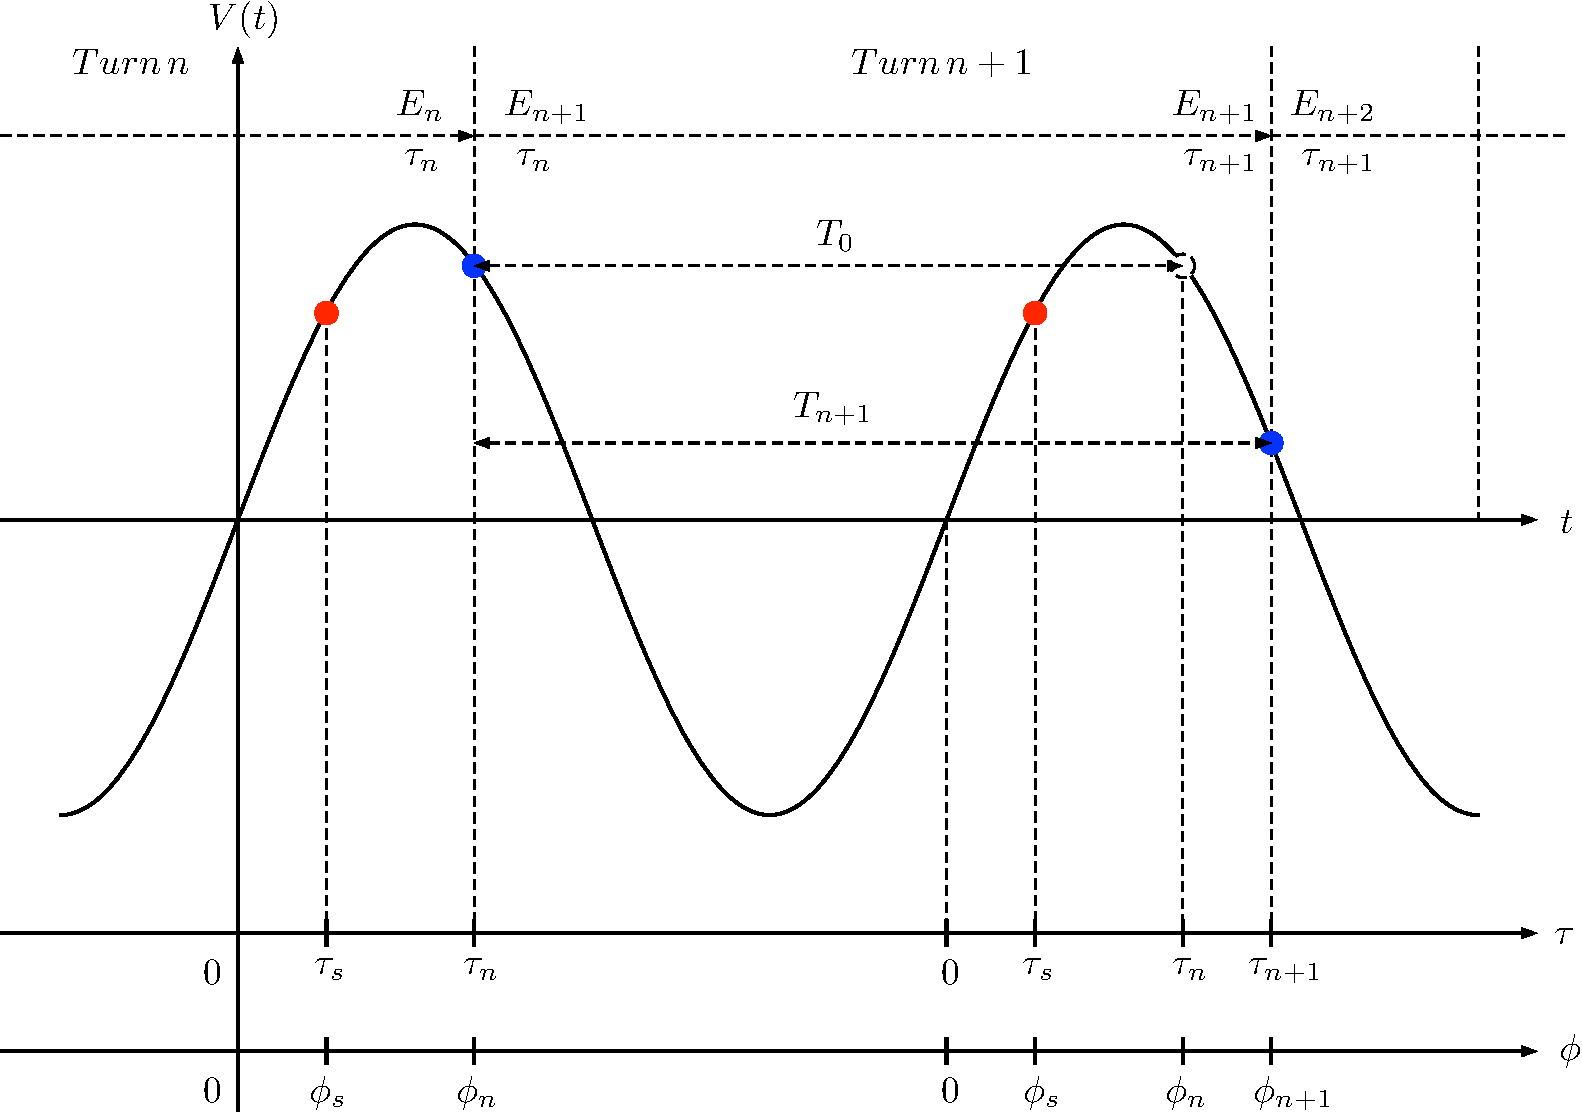
\includegraphics[width=15cm,clip]{coordinates.pdf}
      \caption{Relative and absolute coodinates. ($h=1$)}
      \label{coordinates}
    \end{center}
  \end{figure}

粒子がエネルギー$E_n$でリングを$n$周回し、加速空洞で加速されエネルギーが$E_{n+1}$増えた時、$n+1$周回し再び加速空洞で加速する時間$T_{n+1}$は、
%
\begin{equation}
    \Delta \tau_{n+1} = \tau_{n+1} - \tau_{n} = T_{n+1} - T_{0,n+1}
\end{equation}
%
\begin{equation}
    \phi_{n+1} - \phi_{n} = \omega_{RF} \Delta\tau_{n+1} = \omega_{RF} (T_{n+1}-T_{0,n+1})
\end{equation}
%
\begin{equation}
    \frac{T_{n+1}-T_{0,n+1}}{T_{0,n+1}} = \eta \delta_{n+1}
\end{equation}
%
\begin{equation}
    \phi_{n+1} - \phi_{n} = \omega_{RF} T_0 \eta \delta_{n+1}
\end{equation}
%
以上より、
%
\begin{align}
    \delta_{n+1} - \delta_n &= \frac{e V}{\beta_0^2 E_0}(\sin\phi_n -\sin\phi_s) \\
    \phi_{n+1} - \phi_{n} &= \omega_{RF} T_0 \eta \delta_{n+1}
\end{align}
%
\section{Transverse–Longitudinal Coupling}
\subsection{Dispersion}
運動量偏差 (momentum deviation)
%
\begin{equation}
    \delta_p = \frac{p-p_0}{p_0}=\frac{\Delta p}{p_0}
\end{equation}
%
分散 (dispersion)
%
\begin{equation}
    x(\delta_p) = \left. x \right|_{\delta_p = 0} + \eta_x \delta_p + \eta_x^{(2)}\delta_p^2 + \dots
\end{equation}
%
\subsection{Momentum compaction factor}
momentum compaction factor
%
\begin{equation}
    \alpha_p = \frac{1}{C_0}\left.\frac{dC}{d\delta_p}\right|_{\delta_p = 0}
\end{equation}
%
\subsection{$\delta$ and $\delta_p$}
Note that the momentum deviation $\delta_p$ is not the same as the energy deviation $\delta$. To proceed, it is useful to have a relationship between the derivative with respect to $\delta_p$ and the derivative with respect to $\delta$.
%
\subsubsection{energy deviation}
%
\begin{equation}
    \delta \equiv \frac{E}{P_0 c} -\frac{1}{\beta_0}
\end{equation}
%
$E =\gamma m c^2$, $P_0 =\beta_0\gamma_0 mc$より
%
\begin{align}
    \delta &= \frac{\gamma m c^2}{c(\beta_0\gamma_0 m c)} - \frac{1}{\beta_0} \notag \\
    & = \frac{1}{\beta_0}\left(\frac{\gamma}{\gamma_0} - 1\right) \notag \\
    & = \frac{1}{\beta_0}\left(\frac{E}{E_0}-1\right)
\end{align}
%
\subsubsection{momentum deviation}
%
\begin{equation}
    \delta_p = \frac{P}{P_0} -1
\end{equation}
%
Since $\delta_p = 0$ when $\delta = 0$, we can write:
%
\section{Difference Equations for Longitudinal Motion in a Synchrotron}
The relative time $\tau$ and the relative phase $\phi$ are measured with respect to the zero crossing of the gap voltage. 
%
\begin{equation}
    \tau(n+1) - \tau(n) = T(n+1) -T_0(n+1)
\end{equation}
%
$\phi(n) = \omega_{RF}(n) \tau(n)$と置くと
\begin{align}
    \phi(n+1) &= \omega_{RF}(n+1)\tau(n+1) \notag \\
    &=\omega_{RF}(n+1)\{\tau(n) + T(n+1) -T_0(n+1)\} \notag \\
    &= \frac{\omega_{RF}(n+1)}{\omega_{RF}(n)} \phi(n) + \omega_{RF}(n+1)\{T(n+1) -T_0(n+1)\}  \notag
\end{align}
%
ここで、
%
\begin{equation}
    \frac{T(n+1)-T_0(n+1)}{T_0(n+1)} = \eta \delta_p(n+1)
\end{equation}
%
\begin{align}
    \phi(n+1) &= \frac{\omega_{RF}(n+1)}{\omega_{RF}(n)}\phi(n) + \omega_{RF}(n+1)T_0(n+1)\eta \delta_p(n+1) \notag \\
    &=\frac{\omega_{RF}(n+1)}{\omega_{RF}(n)}\phi(n) + 2\pi h \eta \delta_p(n+1)
\end{align}
%
\begin{equation}
    \frac{\omega_{RF}(n+1)}{\omega_{RF}(n)}\phi(n) \approx 1
\end{equation}
%
\begin{equation}
    \phi(n+1) = \phi(n) + 2\pi h \eta \delta_p(n+1)
\end{equation}

The energy of a particle at the (n+1)-th turn $E(n+1)$ is expressed by the energy $E(n)$ and RF phase $\phi(n)$ at the n-th turn as
%
\begin{equation}
    E(n+1) = E(n) + e V \sin\phi (n)
\end{equation}
%
For a synchronous particle with suffix 0,
%
\begin{equation}
    E_0(n+1) = E_0(n) + e V \sin\phi_s
\end{equation}
%
Thus, the energy error, $\Delta E = E - E_0$, is expressed as
%
\begin{equation}
    \Delta E(n+1) = \Delta E(n) + e V (\sin\phi(n) - \sin\phi_s)
\end{equation}
%
ここで、
%
\begin{equation}
    \delta_p = \frac{\Delta p}{p_0} = \frac{1}{\beta_0^2}\frac{\Delta E}{E_0}
\end{equation}
%
より、
%
\begin{equation}
    \Delta E(n+1) - \Delta E(n) = \beta^2 E_0 \{\delta_p(n+1) - \delta_p(n)\}
\end{equation}
%
したがって、
%
\begin{equation}
    \delta_p(n+1) - \delta_p(n) = \frac{e V}{\beta_0^2 E_0}(\sin\phi(n) -\sin\phi_s)
\end{equation}
%

the symplectic mapping equation:

\begin{align}
    \begin{split}
        &\delta_p(n+1) - \delta_p(n) = \frac{e V}{\beta_0^2 E_0}(\sin\phi(n) -\sin\phi_s) \\
        &\phi(n+1) = \phi(n) + 2\pi h \eta \delta_p(n+1)
    \end{split}
\end{align}
%
\begin{thebibliography}{9}
    \bibitem{Chao}
    A. Chao, K. Mess, M. Tigner, and F. Zimmermann, Handbook of Accelerator Physics and Engineering (2nd Edition), World Scientific Publishing Company Incorporated, Singapore (2013)
    \bibitem{a}
    A.W.Chao and M.Tigner,editors.Handbook of Accelerator Physics and Engineering. World Scientific Pub. Co., 3rd printing edition, 2009.
    \bibitem{Wolski}
    Andy Wolski, Beam Dynamics in High Energy Particle Accelerators,  Imperial College Pr (2014).
    \bibitem{Lee}
    S. Y. Lee, Accelerator physics, World Scientific (2004), ISBN 9789812562005.
    \bibitem{Edwards}
    D.A. Edwards, M.J. Syphers, `An introduction to the physics of high energy accelerators', Wiley (1993).
\end{thebibliography}
%
\end{document}